\chapter{Implementace}
\section{Architektura}
Jak už bylo popsáno, tato práce se zabývá tvorbou dvou klienstkých frameworků pro dvě různé mobilní platformy. Ke správnému fungování frameworků je předpokládána serverova část, která generuje data v určité struktuře a formátu, z nichž oba frameworky umí vytvořit a zobrazit koncovému uživateli prvky grafického uživatelského rozhraní. Použití frameworku na jednotlivých zařízeních zachycuje diagram nasazení na obrázku \ref{img:deploymentDiagram}. Diagram nasazení je určen k tomu, aby zobrazil jak je architektura softwaru namapovaná na architekturu hardwaru. Jedná se o diagram, který patří do implementační fáze, avšak často již vzniká určitá první verze ve fázi návrhové a poté se doplňuje \cite{UmlArlow}.

Obrázek \ref{img:deploymentDiagram} zobrazuje tři zařízení - server, Android klienta a Windows Phone klienta. Pro účely vývoje těchto frameworků byla na serveru nasazena Java EE aplikace AFServer, která za pomocí AFRest \cite{tomasek-thesis} využívající AspectFaces \cite{aspect-faces} generuje definice komponent z modelu, které pak upraví a poskytuje klientovi v požadovaném tvaru, který ji může získat pomocí http dotazu. Android klient interpretuje tuto specifikaci komponenty za pomocí frameworku AFAndroid, který využívá stejných částí jako serverová strana, což zajišťuje kompatibilitu objektů na serverové a klienstké straně. Windows Phone klient interpretuje definici za pomocí AFWinPhone, který bohužel neumožňuje využívat stejných částí se serverem neboť běží na rozdílných platformách. Aby bylo zachováno stejné chování jako u Android klienta, byly tyto části znovu vytvořeny.

Aby klienti mohli framework využívat, musí ho nejdříve vložit. V případě Androidu se framework kompiluje do AAR souboru, který lze do projektů přidat jako Gradle závislost. Gradle je systém pro build projektů a správu závislostí nejen v Androidu. V současné době ho lze využít i v C, C++, Java aplikacích \cite{gradle}. Závislost může být lokální nebo se stahovat z online repozitáře. Jelikož není AFAndroid ještě k dispozici v žádném z online repozitářů, je nutné ho přidat lokálně. To lze udělat přidáním AAR souboru do složky lib nebo vytvořit z knihovny nový modul. Windows Phone framework je zase zkompilován do DLL souboru, který je v současné chvíli nutné také přidat lokálně jako knihovnu mezi reference.

\subsection{Komponenty}
Oba frameworky jsou schopny generovat dva typy komponent - formulář a list. Obě tyto komponenty dědí od třídy AFComponent, která představuje společnou část obou komponent. AFComponent implementuje rozhraní třídy AbstractComponent, která definuje metody pro získání definice komponenty, naplnění daty, generování dat pro odeslání a jejich odeslání na server včetně validace. Tyto metody musí AFComponent nebo některá třída, která od něj dědí, nuceně implementovat. Společná část komponent konkrétně implementuje metody pro získání definice ze serveru a získání dat, kterými se má komponenta naplnit, protože tyto části jsou jak pro formulář, tak pro list identické. Způsob reprezentace komponenty a vložení získaných dat, pak řeší jednotlivé komponenty každá jiným způsobem. Stejně tak list nedisponuje stejnou funkcionalitou jako formulář, je jen pro čtení a proto nepodporuje metody pro generování a následné odesílání dat či jejich validaci. Struktura části Android frameworku zachycující komponenty je na obrázku \ref{img:classDiagramComponents} popsána diagramem tříd. Diagram pro tuto část ve Windows Phone frameworku je až na syntaktické odlišnosti shodný.  

Obě komponenty obsahují metodu, která získá jejich grafickou reprezentaci, kterou pak může vývojář vložit do libovolné části uživatelského rozhraní, neboť tato metoda má návratový typ u Android verze View a u WP verze FrameworkElement, což jsou jedny ze základních prvků GUI na těchto platformách a lze je vložit do jakéhokoliv jiného elementu. V AFSwinx \cite{tomasek-thesis} komponenty rovnou dědily od třídy JPanel a tudíž metodu pro zisk grafické reprezentace nepotřebovaly. Tento přístup však vyústil v to, že se metody poskytované komponentou mísily s nepřeberným množstvím metod příslušících třídě JPanel, což způsobovalo dle uživatelského testu nepřehlednost a zhoršenou orientaci v poskytovaných metodách, proto byl zvolen výše zmíněný přístup. 

Vytvářené komponenty se ve frameworku určitým způsobem ukládají, aby bylo možné je získat a pracovat s nimi v celém programu, ne jen v místě, kde byly vytvořeny. Konkrétně se komponenty skladují ve třídách AFAndroid pro Android a AfWindowsPhone pro WP, zobrazené na obrázku \ref{img:facades}. Tyto třídy jsou implementovány jako singleton, což je návrhový vzor, který se využívá, když je potřeba mít pouze jednu instanci této třídy, ke které lze přistupovat z více míst \cite{gamma}. Singleton často bývá součástí jiných návrhových vzorů jako je napříkald Facade neboli fasáda. Fasáda se používá v případě, že programátor chce poskytnout jednoduché rozhraní pro ovládání složitějšího systému a tím klienty odstínit od vnitřní implementace systém schovaného pod fasádou \cite{gamma}. AFAndroid a AFWinPhone tedy neslouží pouze jako sklad vytvořených komponent ale také jako fasády pro ovládání frameworků. Nabízí získání vytvořené komponenty, jejich smazání, zisk builderů pro tvorbu komponent a nastavení základního skinu, který se použije při sestavování komponent, není-li v při inicializaci builderu specifikováno jinak. Proces sestavení komponenty je složitější proces několika funkcí, které na sebe musí navazovat ve správném pořadí, proto kdyby tyto třídy neexistovaly, nebylo by použití frameworků vůbec snadné.

\begin{figure}[h!]
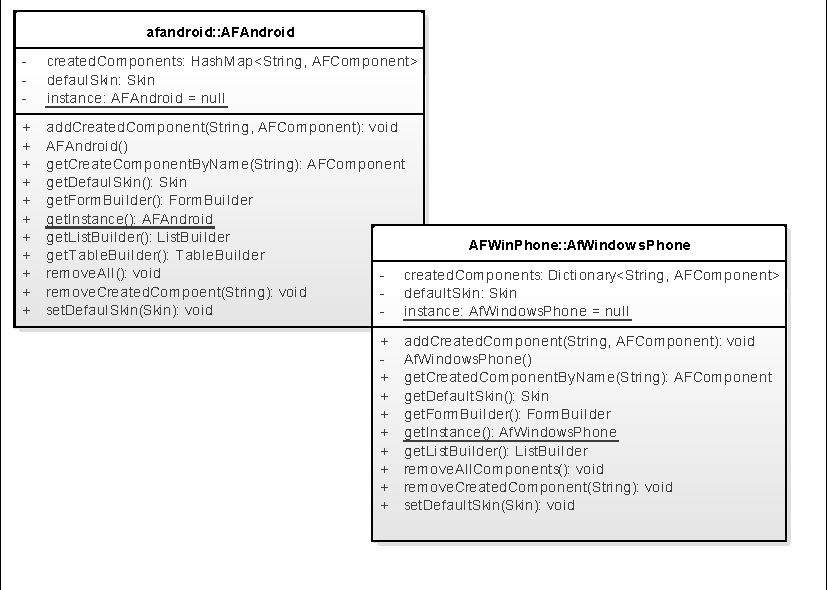
\includegraphics[width=\textwidth]{figures/facades}
\caption{Třídy AFAndroid a AfWindowsPhone sloužící jako fasády pro ovládání frameworků}
\label{img:facades}
\end{figure}

Přiklad vytvoření komponenty v Android frameworku, konkrétně formuláře, za použití fasády AFAndroid je v ukázce kódu \ref{code:createForm}. Kód ukazuje, že je třeba za použití fasády získat builder, který je pak nutné nainicializovat. Inicializace zahrnuje určení zdroje, ze kterého se má definice komponenty získat, definuje InputStream s načteným souborem s definicemi zdrojů a klíč, pod kterým se získá konkrétní připojení. Soubor byl popsán v rámci analýzy a jeho struktura je ukázána v části kódu \ref{code:xmlSource}. Vývojář si komponentu také při inicializaci builderu pojmenuje, tedy přiřadí ji jednoznačný textový řetězec, pod kterým se komponenta uloží do vytvořených komponent a na základě tohoto řetězce ji lze odtud skrz fasádu opět získat. Existuje ještě přetížená metoda pro inicializaci builderu, která je umožnuje přidat dodatečná nastavení pro připojení. Po inicializaci builderu lze nadefinovat ještě skin, který se při vytváření komponenty použije. Jelikož je komponeta vytvářena dynamicky všetně jejích vlastností a vzhledu v rámci metody, která je pro vývojáře zapouzdřená, jediným způsobem jak pohodlně upravit její vzhled je nastavit skin před zahájením její tvorby. Jelikož má vývojář k některým částem komponenty přístup i po jejím vytvoření, lze vzhled komponenty upravit i později, vyžaduje to však znalosti tvorby GUI pro danou platformu, což už je složitější záležitost. Po nastavení skinu lze komponentu vytvořit a dále pak nad ní provádět akce, které poskytuje.  Pro Windows Phone je kód identický, pouze se používá WP fasáda AfWindowsPhone a místo InputStreamu stačí nadefinovat jméno souboru se zdroji, respektive cesta k němu.

Pokud se něco při vytváření nepovede,  například se nelze připojit ke zdroji na serveru, je vyhazována výjimka. Vývojář může výjimku libovolně zpracovat, například zobrazit dialog s chybou.

\begin{lstlisting}[caption=Ukázka tvorby formuláře,
label={code:createForm}, basicstyle=\footnotesize]
InputStream connectionResource = getResources().openRawResource(R.raw.connection);
 try {
	AFForm form = 
		AFAndroid.getInstance().getFormBuilder()
		.initBuilder(getActivity(), LOGIN_FORM_NAME, connectionResource, 
		LOGIN_FORM_CONNECTION_KEY)
		.setSkin(new LoginSkin(getContext()))
		.createComponent();
} catch (Exception e) {
	zpracovani vyjimky, ktera mohla nastat pri vytvareni komponenty
}
\end{lstlisting} 

\section{Komunikace serveru a klienta}
Jak už bylo zmíněno v analýze, server poskytuje zdroje, ze kterých lze získat definice komponent, data nebo na ně lze odeslat uživatelský vstup. K nadefinování těchto zdrojů je potřeba vytvořit XML soubor, který je popsán v ukázce kódu \ref{code:xmlSource}. Tento soubor se zpracuje pomocí příslušného XML parseru a výsledkem je třída AFSwinxConnectionPack, která má v sobě uloženy jednotlivé části daného připojení, kokrétně, kde je uložena definice komponenty, data a kam lze odeslat uživatelský vstup \cite{tomasek-thesis}. V průběhu tvorby komponenty se tyto části připojení využijí k zisku informací, které jsou na definovaných zdrojích, na něž připojení odkazuje, uloženy. Zisk informací je proveden pomocí HTTP požadavku, který vytváří a odesílá třída RequestMaker. Způsob provedení tohoto požadavku je na obou platformách dosti rozdílný, avšak něco mají společného a to, že musí být asynchronní. V mobilních aplikacích se requesty musí provádět asynchroně na jiném vlákně než na hlavním, neboť hlavní vlákno spravuje celé UI aplikace a to by v momentě, kdy se požadavek provádí, zamrzlo, což je nežádoucí. HTTP požadavek v případě, že se získává definice komponenty nebo data, vrací textový řetězec, který obsahuje JSON objekt převedení na textovou reprezentaci, v případě odesílání na server se akce pouze provede.

V Androidu se standartně HTTP requesty řeší v rámci objektu typu AsyncTask \cite{asynctask}, který umožňuje provést akci v pozadí a výsledky akce předat hlavnímu UI vláknu. Tím se vývojáři Android aplikací vyhnou přímé práci s vlákny. Třída RequestMaker od AsyncTask dědí a přetěžuje metodu pro práci v pozadí, kde se celý požadavek vytvoří, odešle a získá se odpověď. Tvorbu a práci s požadavkem má na starosti třída HttpURLConnection, před Android 6.0 by bylo možné ještě použít Apache HttpClient, který byl s příchodem nové verze Androidu smazán. Lze ho po určitém nastavení nadále používat ale ukazuje se, že HttpURLConnection je efektivnější z hlediska využití sítě a spotřeby energie \cite{httpclientremoval}. 

Specifikace požadavku, tj. http metoda, url adresa, data, content-type a případně bezpečnostní omezení, se předávají třídě v konstruktoru. Během procesu se může stát výjimka a jelikož metoda, která pracuje na pozadí nemůže zpropagovat výjimku o úroveň výš, je nutné výjimky řešit v rámci zmíněné metody. Je ale žádoucí ponechat řešení těchto výjimek na vývojáři, proto byla zavedena alternativa, ve které metoda běžící na pozadí vrací Object, který buď může být textový řetězec s daty ze serveru nebo vzniklá výjimka. O úroveň výše tento fakt kontroluje a v případě, že se jedná o výjimku, je vyhozena a zpropagována až k vývojáři. 
Po vytvoření objektu RequestMaker je třeba ho spustit. K tomu slouží metoda executeOnExecutor, která umožňuje spustit v jednu dobu více objektů typy AsyncTask.

WindowPhone verze používá k tvorbě a manipulaci s požadavkem třídu HttpClient \cite{wp-httpclient} v rámci asynchronní metody, která request provádí. V tomto případě problém s propagací případné výjimky až k vývojáři. Nastavení požadavku se provádí přes konstruktor obdobně jako v Android verzi. 

\subsection{Generování komponent}
Na základě definice komponenty, která se ze serveru získá výše uvedeným způsobem, lze generovat komponenty. Typ komponenty, která se vygeneruje závisí na zvoleném builderu. Každý builder je reprezentován třídou, která dědí od abstraktní třídy AFComponentBuilder. Tato třída definuje společné vlastnosti všech builderů a  vynucuje implementaci metody pro vytvoření komponenty jako takové a vytvoření její grafické reprezentace. Proces vytvoření komponenty v Android frameworku je popsán na sekvenčním diagramu v příloze \ref{img:sdFormBuilding}. Proces tvorby ve WP verzi je obdobný s tím rozdílem, že není potřeba znát k vytváření GUI prvků kontext, proto nemusí být do argumetů funkcí předávána aktivita, ve které chceme komponentu vytvořit. Z obrázku je patrné, že po inicializaci builderu a případném nastavení skinu začíná proces tvorby formuláře na jehož konci uživatel získá již hotový formulář. Nejprve dojde k získání metamodelu komponenty ze serveru. Poté začne tvorba jednotlivých polí formuláře, k tomu je zapotřebí odpověď s metamodelem rozparsovat, výsledkem čehož bude třída AFClassInfo obsahující informace o celé komponentě. Tato struktura byla v analytické části popsána na obrázku \ref{img:metadataModel}, skutečná struktura v tomto případě pro Windows Phone framework je na obrázku \ref{img:metadataClass}. AFClassInfo obsahuje 0 až N objektů třídy FieldInfo, tedy objektu držící informace o tvořeném poli. Přes tyto objekty framework iteruje a postupně z nich vytváří objekty třídy AFField, které už obsahují i grafickou reprezentaci pole. 

Při iterování skrze popisy polí je důležité kontrolovat atribut, který určuje zda pole zastupuje v modelu na serveru primitivní nebo složený datový typ. V případě, že se jedná o složený datový typ, vyhledá se k němu v AFClassInfo příslušná definice vnitřní třídy, na kterou se pak funkce, která tvoří jednotlivá pole, rekurzivně zavolá a na místo pole označeného jako vnitřní třída budou vytvořena pole, která jsou nadefinovaná v příslušné vnitřní třídě. 

Součástí tvorby pole není jen nadefinování vlastností a tvorba samotné grafické reprezentace. Při tvorbě formulářových polí je potřeba vytvořit tři elementy, ze kterých se pole skládá - label, místo pro zobrazení validačních chyb a aktivní prvek. To zajišťuje třída FieldBuilder. Vytvořit label a místo pro validační chyby je jednoduché, aktivní prvek je mírně komplikovanější. Součástí třídy FieldInfo je i atribut widgetType, který určuje, jakým typem aktivního prvku má být pole reprezentováno. Na základě tohoto atributu se získává pomocí třídy WidgetBuilderFactory příslušný builder, který umí přímo příslušný aktivní prvek vytvořit. Tento builder poskytuje také funkcionalitu pro získání a nastavení dat vytvořenému aktivnímu prvku. Pro jednoduší přístup k této funkcionalitě, má pole formuláře na builder, který mu vytvořil část s aktivním prvkem, referenci. Po vytvoření všech tří částí se zkompletují do celkové grafické reprezentace, která se poli taktéž nastaví. Takovéto pole se vrátí builderu komponenty, který si jeho existenci zaznamená. Po zaznamenání všech polí, které mají ve formuláři být, se jednotlivé grafické reprezentace polí seskupují do celkového vzhledu komponenty, který se pak komponentě nastaví a vývojář ho potom může z komponenty získat.

\subsubsection{Naplnění komponety daty}
Pokud má být komponenta naplněna daty, je nutné získat jednotlivé buildery, které vytvořily jenotlivá pole. Data se vkládají přímo z odpovědi serveru, která je obsahuje. V datech se objevuje vždy identifikátor daného pole a hodnota, která má být vložena. Dle tohoto identifikátoru je framework shopen vyhledat příslušné pole a z něj získat builder, který postavil jeho aktivní část. Jak už bylo řečeno, builder disponuje funkcí schopnou do pole, které vytvořil, vložit data, což také provede. Takto se to provede u všech polí, která se v přijatých datech vyskytují. Tím je proces tvorby formuláře popsaného na obrázku \ref{img:sdFormBuilding} ukončen a vývojáři je předána vytvořená komponenta. 

\subsubsection{Widget buildery}
Bylo zmíněno, že části formulářových polí, do kterých lze zadat uživatelský vstup, se vytváří pomocí příslušných builderů, jež lze získat pomocí třídy WidgetBuilderFactory. Tato třída využívá návrhový vzor Factory. Ten se využívá, když je potřeba vytvořit objekt a zároveň zastínit logiku vytváření objektu klientovi \cite{factorypattern}. Tento návrhový vzor byl ve frameworku použitý proto, aby se v případě, že by bylo potřeba přidat nový builder, nezasahovalo do logiky vytváření polí, ale pouze do třídy WidgetBuilderFactory. Jednotlivé widget buildery lze vidět na obrázku \ref{img:factoryWidgetBuilders} a jejich seznam je v tabulce \ref{table:widgetBuilders}. Každý builder dědí od základního builderu definovaného abstraktní třídou BasicBuilder implementující rozhraní AbstractWidgetBuilder. AbstractWidgetBuilder definuje metody pro vytvoření grafické reprezentace widgetu, nastavení dat do widgetu a zisk dat z widgetu. Tyto metody musí být pak každým novým builderem implementovány. Ukázka kódu \ref{code:createTextField} zobrazuje tvorbu grafické reprezentace textového pole v Android frameworku.

\begin{lstlisting}[caption=Ukázka tvorby grafické reprezentace textového pole,
label={code:createTextField}, basicstyle=\footnotesize]
@Override
public View buildFieldView(Activity activity) {
    EditText text = new EditText(activity);
    text.setTextColor(getSkin().getFieldColor());
    text.setTypeface(getSkin().getFieldFont());
    addInputType(text, getField().getFieldInfo().getWidgetType());
    if(getField().getFieldInfo().getReadOnly()){
	text.setInputType(InputType.TYPE_NULL);
        text.setTextColor(Color.LTGRAY);
    }
    return text;
}
\end{lstlisting} 

V ukázce \ref{code:createTextField} lze vidět, že na vstupní pole je aplikován skin, který upravuje jeho vzhled. Konkrétně v případě textového pole se nastavuje barva jeho textu a typ písma.

\begin{table}[h!]
\begin{center}
\caption{Podporované widget buildery}
\label{table:widgetBuilders}
\begin{tabular}{|p{4cm}|p{3cm}|p{7cm}|}
\hline
\textbf{Builder} & \textbf{Typ widgetu} & \textbf{Popis} \\
\hline
DateWidgetBuilder & 
Calendar & Používá se při reprezentaci atributů typu datum. Umožní uživateli zobrazit date picker, pomocí kterého lze vybrat datum. \\
\hline
DropDownWidgetBuilder &
dropDownMenu & Menu, ze kterého lze vybrat jednu z několika voleb. \\
\hline
CheckBoxWidgetBuilder & checkBox &
Zaškrtávací políčko reprezentující hodnotu true nebo false podle toho, zda je nebo není zaškrtnuto. \\
\hline
TextWidgetBuilder & textField &
Builder pro textové pole. Lze mu nastavit typ vstupu, podle kterého se změní klávesnice pro zadávání znaků například na číselnou. V Android frameworku lze použít i pro pole s heslem. \\
\hline
PasswordWidgetBuilder & password &
Pole pro hesla. Text, který uživatel dovnitř napíše je převeden na zástupné znaky. Tento builder se vyskytuje pouze ve WP verzi frameworku, Android verze k tomuto účelu používá TextWidgetBuilder \\
\hline
OptionBuilder & option &
Vytvoří skupinu radiobuttonů, z které lze vybrat jednu hodnotu. Pokud nejsou definovány možnosti vytvoří se 2 radiobuttony s hodnotami ano a ne \\
\hline
\end{tabular}
\end{center}
\end{table}

\subsubsection{Skiny}
Skiny neupravují pouze vzhled aktivního prvku, ale také vzhled labelu, validačních chyb nebo i celé komponenty. Lze nastavit grafické vlastností jako je barva textu, pozadí, velikost textu a jeho font, ale také rozměry celé komponenty. Ve frameworcích existuje rozhraní Skin, které deifnuje všechny nastavitelné vlastnosti. Už bylo zmíněno, že skiny se musí nastavit před tvořením komponenty jejímu builderu. Toto nastavení je ale volitelné a tak existuje třída DefaultSkin, která toto rozhraní implementuje a definuje základní vzhled, který se použije nespecifikuje-li vývojář jinak. Vývojář pravděpodobně nebude chtít předělat úplně celý vzhled, ale ppuze některé části skinu. K tomuto mu stačí dědit od třídy DefaultSkin a pouze přetížit metody udávající vlastnosti, které chce změnit.

\subsubsection{Layouty}
Při vytváření grafické reprezentace komponenty, server definuje, jak se její jednotlivé části v rámci komponenty uspořádají. V případě formuláře je nutné uspořádat pole tak, aby byl formulář přehledný a dobře použitelný. V případě listu jde hlavně o přehlednost, neboť jednotlivé položky listu by byly při větším obsahu moc vysoké a nevzhledné. Server definuje osu, podle které jsou komponenty vykreslovány, počet sloupců a pozici labelu \cite{tomasek-thesis}. Layout lze určit buď celé komponentě, ten na obrázku \ref{img:metadataClass} reprezentován třídou TopLevelLayout nebo pouze části komponenty tj. poli, který je na obrázku reprezentován třídou Layout. V případě layoutu komponenty je pouze definována osa a počet sloupců, layout jednotlivých polí přidává pozici labelu. Hodnoty, kterých jednotlivé vlastnosti nabývají jsou popsány pomocí následujících výčtových typů, které lze vidět i na obrázku \ref{img:metadataClass}.
\begin{itemize}
\item LayoutDefinitions, který určuje počet sloupců a nabývá hodnot ONECOLUMNLAYOUT a TWOCOLUMNSLAYOUT, tedy jednosloupcové a dvousloupcové rozložení.
\item LayoutOrientation, který určuje osu, ve směru které se části komponenty vykreslují. Nabývá hodnot AXISX a AXISY, první určuje směr vykreslování podle osy X, druhá podle osy Y.
\item LabelPosition, který určuje pozici labelu vzhledem k aktivnímu prvku. Nabývá hodnot BEFORE, AFTER a NONE. První znamená, že bude label před aktivním prvkem, druhá za aktivním prvkem a třetí znamená, že label nebude vůbec zobrazen.
\end{itemize}

Layouty jsou v jednotlivých klientských frameworcích interpretovány různě. Zatímco v případě Android frameworku je layout realizován pomocí seskupení LinearLayoutů \cite{android-lin-layout}, WP verze používá k tvorbě layoutu Grid \cite{wp-grid}. Důvodem není nic zvláštního, k oběma třídám existují na druhé platformě ekvivalenty, pomocí kterých lze dosáhnout stejných výsledků, jde spíše o to, ukázat více možných způsobů implementace. 

Důležitým aspektem je také pořadí jednotlivých částí komponenty. To definuje server a v metadatech se informace o polích objeví už v daném pořadí, které je třeba zachovat. Proto bylo nutné použít k uskladnění kolekci, která zachovává pořadí svých prvků, takovou je například List \cite{tomasek-thesis}.

\subsubsection{Lokalizace}
Jelikož se mohou v metadatech objevit i texty pro překlad, bylo třeba naimplementovat třídu Localization, která se stará o překlady těchto textů. Třída disponuje samoutnou funkcí pro překlad a funkcí pro změnu jazyku. V Androidu se typicky lokalizační texty umisťují do souboru strings.xml ve složce values. Pro Windows Phone je to obdobné. Zde se texty vkládají do souborů Resources.resw, které jsou umístěny ve složce s názvem jazyku ve složce Strings. S tímto umístěním textů oba frameworky počítají, u Android verze je sice možnost nadefinovat jiný balíček, ve kterém by se texty měly hledat, ale stále se předpokládá umístění ve values/strings.xml. Třída Localization se dá využít i pro překlad jiných textů i mimo framework a to i v rámci XML šablon, ve kterých je vytvořeno statické UI. Při startu aplikace se použije jazyk zařízení. Pokud by pro daný jazyk neexistovaly předklady, je vhodné mít defaultní soubory s texty, které se v tomto případě použijí.

\subsection{Práce s komponentami}
Vytvořená komponenta disponuje různými funkcemi, které umožňují s ní dále pracovat. Pro formulář jsou to metody pro odeslání, validaci, resetování nebo vyčištění formuláře. List je komponenta, která by měla pouze zobrazovat data, proto s ní nejde provést ani moc akcí. Obsahuje však důležitou funkci, pomocí které lze získat obsah jedné položky listu, který lze pak využít například pro naplnění formuláře. 

Nejdůležitější funkcí je však odeslání formuláře, který je zobrazen na sekvenčním diagramu \ref{img:sdFormSend}. K tomuto účelu má formulář metodu sendData. V rámci této metody se nejdříve zjistí, zda vývojář pro komponentu nadefinoval v XML souboru s připojeními část označenou uzlem <send>, který definuje, kam se budou data odesílat a jehož struktura lze vidět v ukázce kódu \ref{code:xmlSource}. Komponenty mají atribut connectionPack typu AFSwinxConnectionPack, který obsahuje všechna definována připojení. V případě, že vývojář specifikoval uzel <send> se v tomto atributu formuláře objeví i připojení na zdroj, který přijímá uživatelský vstup. Pokud připojení nadefinované není vyhodí se výjimka, která je propagována k vývojáři, který s ní dle svého uvážení naloži. Pokud připojení existuje, vygenerují se z formuláře data ve formátu, které server dokáže zpracovat. Klient nezná přesně objekty, které se odeslání na serveru vytvoří či upraví, zná ale jejich strukturu, která stačí k tomu, aby byla vytvořena data, která server dokáže přijmout. V rámci generování dat proběhne nejdříve jejich validace, která je blíže popsána v sekci níže. Pokud data nejsou validní vrací metoda sendData hodnotu false, která určuje, že se odesílání nezdařilo. Samotný proces generování dat byl převzat z frameworku AFSwinx. Ten využívá pro znovupostavení dat object typu BaseRestBuilder disponující metodou reserialize. \cite{tomasek-thesis}. BaseRestBuilder je implementován prozatím jen třídou JSONBuilder, která dokáže z formuláře vytvořit JSON soubor a použije se v případě, že server požaduje JSON formát. Další formáty nejsou prozatím podporovány. Metoda reserialize, kterou builder dat používá, již očekává vyparsovaná data z komponenty uložená v objektu typu AFDataHolder. Vytvoření těchto dat provádí komponenta sama. Uživatelský vstup získává z aktivní prvků, ke kterým má skrz kolekci polí typu AFField přístup. Data se získávají z aktivního prvku pomocí widget builderu, který aktivní prvek vytvořil a na který má AFField referenci.  Každý AFField má svůj unikátní identifikátor, který lze využít pro zjištění pozice proměnné v objektu na serveru, který má odeslání formuláře ovlivnit. Pokud indentifikátor obsahuje tečku, znamená to, že dané pole je částí reprezentace neprimitivního datového typu, tedy vnitřní třídy a k té je třeba hodnotu promenné přidat. Pokud v identifikátoru tečka není, znamená to, že jsme na správném místě a do mapy AFDataHolder se přidá nová proměná s hodnotou \cite{tomasek-thesis}. Android verze využívá již naimplementovaný JSON Builder, který využívá k sestavení dat framework GSON \cite{gson}.Ve Windows Phone verzi musel být builder dat přepsán a využívá Windows knihovnu pro práci s JSON soubory. Po vytvoření dat stačí data odeslat na definovaný zdroj na serveru pomocí třídy RequestMaker, která byla popsána výše. Jak už bylo zmíněno, v rámci procesu odeslání může dojít k výjimkám, které jsou předány vývojáři ke zpracování. 

Odeslání formuláře je tedy jednoduché, stačí definovat zdroj v XML souboru a pak například jako reakci na stiknutí tlačítka zavolat metodu sendData. Dále je nutné, aby aplikace nespadla, ošetřit výjimky, které mohou při odesílání nastat. V případě, že nenastane žádná výjimka, data jsou validní a povede se je z formuláře vygenerovat, může vývojář navázat na odeslání další akci. Vývojáři je tedy celý proces odeslání schován a nemusí se jím vůbec zabývat, díky čehož je použití frameworku snadné. Nevýhodou však je, že je vývojář omezen na použití nabízených funkcí frameworku a nemůže do procesu odeslání nijak zasahovat \cite{tomasek-thesis}. 

Dalšími funkcemi, které formulář nabízí je resetování a vyčištění formuláře. Reset formuláře provede obnovení aktuálních dat ve formuláři. Pokud je tedy formulář naplněn nějakými daty a uživatel data změní, lze se k původním nezměneným datům před odesláním formuláře vrátit. Vyčištění formuláře pak nastaví aktivní prvky formuláře na prázdné.

\subsubsection{Validace a Validátory}